
\section{Experiments}
\label{sec:experiments}


\begin{table}
\footnotesize
\begin{tabular}{cccccc}
\toprule
Model & RT & SST & SST & IMDB & Time \\
& & fine & bin & & (s)\\
\midrule
\footnotesize DAN-ROOT & --- & 46.9 & 85.7 & --- & \bf 31\\
\footnotesize DAN-RAND & 77.3 & 45.4 & 83.2 & 88.8 & 136\\
\footnotesize DAN & 80.3 & 47.7 & 86.3 & 89.4 & 136\\
\midrule
\footnotesize NBOW-RAND & 76.2 & 42.3 & 81.4 & 88.9 & 91 \\
\footnotesize NBOW & 79.0 & 43.6 & 83.6 & 89.0 & 91 \\
\footnotesize BiNB & --- & 41.9 & 83.1 & --- & ---\\
\footnotesize NBSVM-bi & 79.4 & --- & --- & 91.2 & ---\\
\midrule
\footnotesize RecNN$^*$ & 77.7 & 43.2 & 82.4 & --- & --- \\
\footnotesize RecNTN$^*$ & --- & 45.7 & 85.4 & --- & --- \\
\footnotesize DRecNN & --- & 49.8 & 86.6 & --- & 431\\
\footnotesize TreeLSTM & --- & \bf 50.6 & 86.9 & --- & --- \\
\footnotesize DCNN$^*$ & --- & 48.5 & 86.9 & 89.4 & ---\\
\footnotesize PVEC$^*$ & --- & 48.7 & 87.8 & \bf 92.6 & --- \\
\footnotesize CNN-MC & \bf 81.1 & 47.4 & \bf 88.1 & --- & 2,452 \\
\footnotesize WRRBM$^*$ & --- & --- & --- & 89.2 & ---\\
\bottomrule
\end{tabular}
\caption{\dan s achieve comparable sentiment accuracies to syntactic functions (bottom third of table) but require much less training time (measured as time of a single epoch on the \abr{sst} fine-grained task). Asterisked models are initialized either with different pretrained embeddings or randomly.}

\label{table:sentiment}
\end{table}

We compare \dan s to both the shallow \nbow\ model as well as more complicated
syntactic models on sentence and document-level sentiment analysis and factoid
question answering tasks. The \dan\ architecture we use for each task is almost
identical, differing across tasks only in the type of output layer and the
choice of activation function. Our results show that \dan s outperform other
bag-of-words models and many syntactic models with very little training
time.\footnote{Code at \url{http://github.com/miyyer/dan}.} On the
question-answering task, \dan s effectively
train on out-of-domain data, while \recnn s struggle to reconcile the syntactic
differences between the training and test data.

\subsection{Sentiment Analysis}\label{sec:sst}

Recently, syntactic composition functions have revolutionized both fine-grained
and binary (positive or negative) sentiment analysis. We conduct sentence-level
sentiment experiments on the Rotten Tomatoes (\abr{rt}) movie reviews
dataset~\cite{pang2005seeing} and its extension with phrase-level labels, the
Stanford Sentiment Treebank (\abr{sst}) introduced
by~\newcite{socher2013recursive}. Our model is also effective on the
document-level \abr{imdb} movie review dataset of~\newcite{maas2011}.

\subsubsection{Neural Baselines}

Most neural approaches to sentiment analysis are variants of either recursive or
convolutional networks. Our recursive neural network baselines include standard
\recnn s~\cite{SocherEtAl2011:RAE}, \rntn s, the deep recursive network
(\drnn) proposed by~\newcite{irsoy-drsv}, and the \tlstm\ of~\cite{taiacl15}. Convolutional network baselines
include the dynamic convolutional
network~\cite[\dcnn]{kalchbrenner2014convolutional} and the convolutional neural
network multi-channel~\cite[\cnnmc]{kim:2014:EMNLP2014}. Our other neural
baselines are the sliding-window based paragraph
vector~\cite[\pvec]{le2014distributed}\footnote{\pvec\ is computationally
  expensive at both training and test time and requires enough memory to store a
  vector for every paragraph in the training data.} and the word-representation
restricted Boltzmann machine~\cite[\wrrbm]{dahl2012training}, which only works
on the document-level~\abr{imdb} task.\footnote{The~\wrrbm\ is trained using a
  slow Metropolis-Hastings algorithm.}

\subsubsection{Non-Neural Baselines}

We also compare to non-neural baselines, specifically the bigram na\"ive Bayes
(\binb) and na\"ive Bayes support vector machine (\nbsvm) models introduced by
\newcite{sidaw12simple}, both of which are memory-intensive due to huge feature
spaces of size $|V|^2$.

\subsubsection{DAN Configurations}

In Table~\ref{table:sentiment}, we compare a variety of \dan\ and
\nbow\ configurations\footnote{Best hyperparameters chosen by cross-validation:
  three 300-d ReLu layers, word dropout probability $p=0.3$, L2 regularization
  weight of 1e-5 applied to all parameters} to the baselines described above. In
particular, we are interested in not only comparing \dan\ accuracies to those of
the baselines, but also how initializing with pretrained embeddings and
restricting the model to only root-level labels affects performance. With this
in mind, the \nbowr\ and \danr\ models are initialized with random
300-dimensional word embeddings, while the other models are initialized with
publicly-available 300-d \texttt{GloVe} vectors trained over the Common
Crawl~\cite{glove2014}.  The \danroot\ model only has access to sentence-level
labels for \abr{sst} experiments, while all other models are trained on labeled
phrases (if they exist) in addition to sentences. We train all \nbow\ and
\dan\ models using AdaGrad~\cite{duchi2011adaptive}.

We apply \dan s to documents by averaging the embeddings for all of a document's
tokens and then feeding that average through multiple layers as before. Since
the representations computed by \dan s are always $d$-dimensional vectors
regardless of the input size, they are efficient with respect to both memory and
computational cost. We find that the hyperparameters selected on the \abr{sst}
also work well for the \abr{imdb} task.

\subsubsection{Dataset Details}

We evaluate over both fine-grained and binary sentence-level classification
tasks on the \abr{sst}, and just the binary task on \abr{rt} and \abr{imdb}. In
the fine-grained \abr{sst} setting, each sentence has a label from zero to five
where two is the neutral class. For the binary task, we ignore all neutral
sentences.\footnote{Our fine-grained \abr{sst} split is \{train: 8,544, dev:
  1,101, test: 2,210\}, while our binary split is \{train: 6,920, dev:872,
  test:1,821\}. Split sizes increase by an order of magnitude when labeled
  phrases are added to the training set. For \abr{rt}, we do 10-fold CV over a
  balanced binary dataset of 10,662 sentences. Similarly, for the \abr{imdb}
  experiments we use the provided balanced binary training set of 25,000
  documents.}

\subsubsection{Results}

The \dan\ achieves the second best reported result on the \abr{rt} dataset,
behind only the significantly slower \cnnmc\ model. It's also competitive with more complex models on the \abr{sst} and outperforms
 the \dcnn\ and \wrrbm\ on the document-level \abr{imdb}
task. Interestingly, the \dan\ achieves good performance on the \abr{sst} when
trained with only sentence-level labels, indicating that it does not suffer from
the vanishing error signal problem that plagues \recnn s. Since acquiring
labelled phrases is often expensive~\cite{sayeed-12,IyyerEtAl2014}, this result
is promising for large or messy datasets where fine-grained annotation is
infeasible.

\subsubsection{Timing Experiments}

\dan s require less time per epoch and---in general---require fewer epochs than
their syntactic counterparts. We compare \dan\ runtime on the \abr{sst} to
publicly-available implementations of syntactic baselines in the last column of
Table~\ref{table:sentiment}; the reported times are for a single epoch to
control for hyperparameter choices such as learning rate, and all models use
300-$d$ word vectors. Training a \dan\ on just sentence-level labels on the
\abr{sst} takes under five minutes on a single core of a laptop; when labeled
phrases are added as separate training instances, training time jumps to twenty
minutes.\footnote{We also find that \dan s take significantly fewer epochs to
  reach convergence than syntactic models.} All timing experiments were performed on a
single core of an Intel I7 processor with 8GB of RAM.



\subsection{Factoid Question Answering}


\begin{table}[t]
\begin{center}
\begin{tabular}{lrrrr}
\toprule
Model    & Pos 1 & Pos 2 & Full & \footnotesize Time(s) \\
\midrule
BoW-DT & 35.4 & 57.7 & 60.2 & --- \\
IR & 37.5 & 65.9 & 71.4 & N/A \\
QANTA & 47.1 & 72.1 & 73.7 & 314 \\
DAN & 46.4 & 70.8 & 71.8 & \bf 18 \\
\midrule
IR-WIKI & 53.7 & \bf 76.6 & \bf 77.5 & N/A\\
QANTA-WIKI & 46.5 & 72.8 & 73.9 & 1,648 \\
DAN-WIKI & \bf 54.8 & 75.5 & 77.1 & 119 \\
\bottomrule
\end{tabular}

\end{center}
\caption{The \dan\ achieves slightly lower accuracies than the more complex \qanta\ in much less training time, even at
  early sentence positions where compositionality plays a bigger role. When Wikipedia is added to the training set (bottom half of table), the \dan\ outperforms \qanta\ and achieves comparable accuracy to a state-of-the-art information retrieval baseline, which highlights a benefit of ignoring word order for this task.}
\label{table:qb}
\end{table}

\begin{figure}	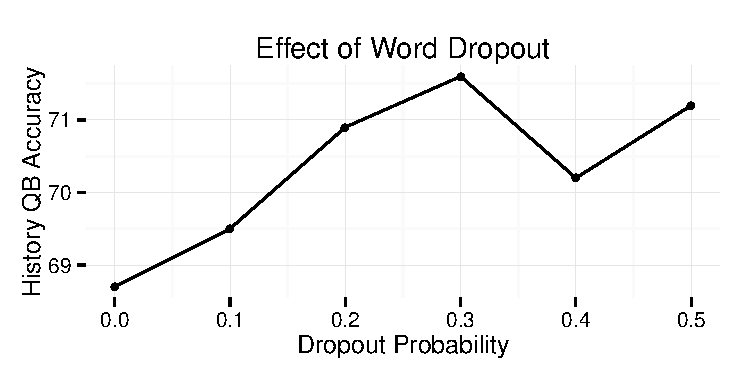
\includegraphics[scale=0.6]{2015_acl_dan/figures/dropout_effect.pdf}
	\caption{Randomly dropping out 30\% of words from the vector average is
          optimal for the quiz bowl task, yielding a gain in absolute accuracy
          of almost 3\% on the quiz bowl question dataset compared to the same model trained with no word dropout.}
\label{fig:sdrop}

\end{figure}

\dan s work well for sentiment analysis, but how do they do on other \abr{nlp}
tasks?  We shift gears to a paragraph-length factoid question answering task and
find that our model outperforms other unordered functions as well as a more
complex syntactic \recnn\ model. More interestingly, we find that unlike the
\recnn, the \dan\ significantly benefits from out-of-domain Wikipedia training
data.



Quiz bowl is a trivia competition in which players are asked
four-to-six sentence questions about entities (e.g., authors, battles,
or events). It is an ideal task to evaluate \dan s because there is
prior work using both syntactic and unordered models for quiz bowl
question answering. In \newcite{Boyd-Graber:Satinoff:He:III-2012},
na\"{\i}ve Bayes bag-of-words models ({\bf \textsc{bow-dt}}) and sequential language models
work well on easy questions but poorly on harder ones. A
dependency-tree \recnn\ called \qanta\ proposed
in~\newcite{IyyerQA2014} shows substantial improvements, leading to
the hypothesis that correctly modeling compositionality is crucial for answering
hard questions.

\subsubsection{Dataset and Experimental Setup}

To test this, we train a \dan\ over the history questions from
\newcite{IyyerQA2014}.\footnote{The training set contains 14,219 sentences over
  3,761 questions. For more detail about data and baseline systems,
  see~\newcite{IyyerQA2014}.} This dataset is augmented with 49,581
sentence/page-title pairs from the Wikipedia articles associated with the
answers in the dataset. For fair comparison with \qanta, we use a normalized
tanh activation function at the last layer instead of ReLu, and we also change
the output layer from a softmax to the margin ranking
loss~\cite{weston2011wsabie} used in \qanta. We initialize the \dan\ with the same pretrained 100-d word embeddings that were used to initialize \qanta.

We also evaluate the effectiveness of word dropout on this task in
Figure~\ref{fig:sdrop}. Cross-validation indicates that $p=0.3$ works best for question answering, although the improvement in
accuracy is negligible for sentiment analysis. Finally, continuing the trend observed in
the sentiment experiments, \dan\ converges much faster than \qanta.

\subsubsection{DANs Improve with Noisy Data}

Table~\ref{table:qb} shows that while \dan\ is slightly worse than \qanta\
when trained only on question-answer pairs, it improves when trained on
additional out-of-domain Wikipedia data (\danw), reaching performance comparable
to that of a state-of-the-art information retrieval system (\irw). \qanta, in
contrast, barely improves when Wikipedia data is added (\qantaw) possibly due to
the syntactic differences between Wikipedia text and quiz bowl question text.

The most common syntactic structures in quiz bowl sentences are imperative
constructions such as ``Identify this British author who wrote Wuthering
Heights'', which are almost never seen in Wikipedia. Furthermore, the subject of
most quiz bowl sentences is a pronoun or pronomial mention referring to the
answer, a property that is not true of Wikipedia sentences (e.g., ``Little of
Emily's work from this period survives, except for poems spoken by
characters.''). Finally, many Wikipedia sentences do not uniquely identify the
title of the page they come from, such as the following sentence from Emily
Bront{\"e}'s page: ``She does not seem to have made any friends outside her
family.'' While noisy data affect both \dan\ and \qanta, the latter is
further hampered by the syntactic divergence between quiz bowl questions and
Wikipedia, which may explain the lack of improvement in accuracy.


